\chapter{Neuronové sítě}
\label{sec:NN}

Umělá neuronová síť (ang. Artificial Neural Network - ANN) nebo jen neuronová
síť (ang. Neural Network - NN) je výpočetní model inspirovaný biologickými
nervovými systémy v lidském mozku. Na rozdíl od konvenčních výpočetních modelů,
které zpracovávají informace algoritmicky, a tedy postupují dle předem určeného
postupu, se informace v tomto modelu šíří paralelně v síti váh mezi
jednotlivými neurony. Jelikož je výstup ze sítě dané architektury závislý
hlavně na numerických parametrech, zejména váhách jednotlivých spojů mezi
neurony, lze funkčnost sítě měnit bez změny programu pouhou změnou těchto
parametrů, a to i automaticky v procesu trénování modelu.

Nyní krátce projdeme historií vývoje neuronových s síti.

\section{Historie}
\label{sec:NN_History}

\subsection{Prvopočátky}
První matematický model neuronové sítě byl popsán v roce 1943 dvěma
neurofyziology - Warrenem McCullochem a Walterem Pittsem. \cite{McCulloch1943}
Model byl založen na síti jednoduchých logických prvků, které provedou vážený
součet svých vstupů a na výstup odešle signál založený na prahové funkcí.

V roce 1958 pak Frank Rosenblatt představil elektronicky model neuronové sítě.
Základní jednotku, postavenou na McCulloch-Pittsově modelu, nazval perceptron.
\cite{Rosenblatt1958} Jeho architektura byla podobná modelu znázorněnému na
obrázku \ref{fig:neuron}, kde aktivační funkce je prahová funkce. Rosenblattův
stroj - Mark I Perceptron - byl postavený pro rozpoznávání jednoduchých vzorů v
obrazech. Hlavním omezením tohoto modelu bylo, že byl schopen rozlišovat pouze
lineárně separovatelné třídy. Samotný model perceptronu je dodnes používán jako
základ pro mnoho neuronových síti.

Další systém - ADALINE (Adaptive Linear Neuron) - byl představen Bernardem
Widrowem and Tedym Hoffem v roce 1960. Tento model umělého neuronu byl velmi
podobný perceptronu, na rozdíl od něj ale neobsahoval prahovou ale lineární
funkcí, výstup tedy nebyl binární ale spojitý. Pro učení pak byla využitá
metoda nejmenších čtverců, která minimalizovala chybu mezi skutečným a
očekávaným výstupem. \cite{nn_history}

I když ve svých počátcích přitahoval koncept umělé inteligence mnoho vědců jako
i sponzorů, v následujících létech zájem ochabl, jelikož nebylo dosaženo
předpokládaných výsledků, hlavně s ohledem na tehdejší stav vývoje hardwaru a
obecně výpočetní techniky. Proto se tomuto období někdy říká Ai Winter.
Neznamená to ale, že ti, kteří se oboru nadále věnovali, nedosáhli významných
výsledků. \cite{nn_history}

\subsection{Backpropagation}
Významným milníkem v historii neuronových sítí byl objev algoritmu
backpropagation, zvaného taky algoritmus zpětného šíření chyby. Tento
algoritmus byl vyvinut v roce 1974 Paulem Werbosem, popularitu ale dosáhl až po
nezávislém objevení v roce 1986 Davidem Rumelhartem et al.
\cite{backpropagation}

Tento algoritmus umožnil trénovat sítě s více vrstvami, což položilo základ
hlubokému učení. Algoritmus využívá metodu gradientního sestupu v kombinaci s
řetězovým pravidlem derivací k nalezení optimálních vah sítě vedoucích k
minimalizaci chyby.

Vynález backpropagation byl jedním z hlavních důvodů, proč se v 80. letech
obnovil zájem o neuronové sítě a umělou inteligenci obecně.

\section{Struktura neuronové sítě}

Umělé neuronové sítě jsou silně inspirovaný biologickými neuronovými sítěmi. A
i když napodobení celé funkčnosti lidského nervového systému by bylo velmi
složité - ne-li nereálné, zejména s ohledem na počet neuronů a způsob jejích
propojení, je možné simulovat alespoň některé funkce lidské mysli.

Pro provádění výpočtů využívají neuronové sítě distribuovaný, paralelní
přístup. Informace jsou tedy zpracovány, předávaný a ukládány celou sítí,
nikoliv pomocí určitých paměťových buněk. Většina znalosti je uložena v sílách
vazeb mezi jednotlivými neurony. Vazby, které vedou k úspěšnému řešení problému
jsou posilovány, naopak ty, které vedou k neúspěchu jsou oslabovány.

Podstatnou vlastností neuronových sítí je jejich schopnost učení. Tato
vlastnost způsobuje, že již není nutná algoritmizace řešené úlohy, ale stačí
neuronové síti opakovaně předložit příklady popisující daný problém, podle
kterých jsou postupně upravovány síly vazeb v síti. Tato fáze učení pak určuje,
jakým způsobem bude síť transformovat vstupní data na
výstupní.\cite{Vondrak1994}

\subsection{Neuron}
Biologický neuron se skládá ze tří hlavních části. Dendrity přijímají vstupní
signály. V těle jsou vstupní signály sečteny do jednoho potenciálu, který vede
k vybuzení neuronu - zaslání signálu na výstup, pokud potenciál překročí
určitou mez. Axanové vlákno pak vede k synapsím, tedy spojům s dalšími neurony.
Lidská mysl pak funguje na principu posilování nebo oslabování těchto spojů.

Umělý neuron se snaží tuto funkčnost napodobit, viz obrázek \ref{fig:neuron}.
Jeho vstupy $x_i$ jsou násobeny váhami $w_i$, které reprezentují sílu daného
spoje. Neuron pak tyto vážené vstupy sečte, a na tento součet aplikuje
aktivační funkci, který definuje hodnotu výstupu $y$. V prvním a základním
modelu neuronu, perceptronu, je aktivační funkcí prahová funkce s binárním
výstupem. Nicméně v praxi se dnes využívají většinou reálné hodnoty a aktivační
funkce je obvykle spojitá. \cite{Vondrak1994} Existuje mnoho různých
aktivačních funkcí, některé z nich budou popsány v další části.

Kromě váh jednotlivých vstupů neuron obvykle obsahuje ještě tzv. bias (někdy
taky prah nebo posun), kterého funkci je posunout vážený součet vstupů tak, aby
bylo možné modelovat i funkce, které nejsou nulové v počátku souřadnic. Je buď
reprezentován jako samostatný parameter, nebo jako váha konstantního vstupu s
hodnotou 1, jako na obrázku \ref{fig:neuron}.

Funkci umělého neuronů lze tedy formálně vyjádřit takto:
\begin{equation}
    y=f\left(\sum_{i=0}^{n}w_{i}x_{i}\right)
\end{equation}
kde $w_0$ je bias a $x_0=1$, anebo s osamostatněným biasem takto:
\begin{equation}
    y = f\left(\sum_{i=1}^{n} w_i x_i + b\right)
\end{equation}
kde $b$ je bias.

Obecně tvoří všechny vstupní váhy a bias množinu parametrů, které ovlivňují
funkčnost celé neuronové sítě. Proces trénování sítě pak spočívá v nalezení
optimálních hodnot těchto parametrů, které vedou k co nejmenší chybě při řešení
úlohy.

\subsection{Základní aktivační funkce}

Aktivační funkce hraje stěžejní roli v umělých neuronových sítích zavedením
nelinearity do celého systému a umožňuje tak učení se složitějších vzorců.

V průběhu let bylo vyvinuto mnoho typů aktivačních funkcí, a i když jejich
úloha se zdá být podobná, můžou se od sebe výrazně lišit. Jejich rozdíly
spočívají zejména v oboru hodnot, spojitosti, monotonnosti, a v tom, zda je
závislá na přídavných trénovaných parametrech. Ve výsledku se taky liší i
jejích využití. Nyní projdeme několik základních aktivačních funkcí, od kterých
se většina ostatních nějakým způsobem odvíjí.

\subitem{Sigmoida (lineární křivka)}

Tato funkce transformuje vstup do rozmezí 0 ÷ 1, je tak vhodná pro odhad
pravděpodobnosti. Proto se taky někdy používá pro ve výstupních vrstvách síti.
Její nevýhodou je hlavně problém mizejícího gradientu, který způsobuje zamezení změny parametrů 

\begin{equation}
    f(x)= \frac{1}{1+e^{-x}}
\end{equation}

\subsection{Dělení neuronových sítí}

\begin{figure}[]
    \centering
    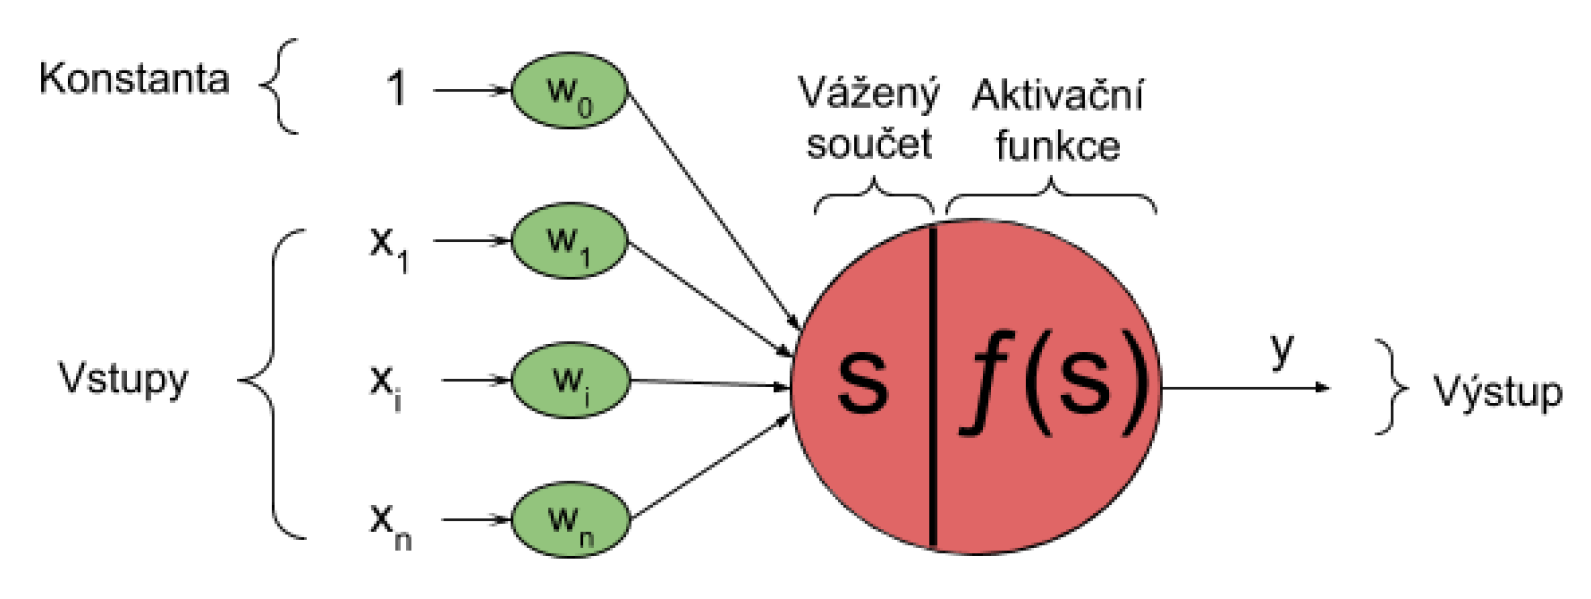
\includegraphics[width=0.5\textwidth]{Figures/neuron.png}
    \caption{Model umělého neuronu \cite{lagan}}
    \label{fig:neuron}
\end{figure}

\endinput